\section{Introducción}
En este capítulo presento la metodología que enmarca los experimentos realizados. Tomando como base la metodología \textit{\acrfull{CRISP-DM}} divido el trabajo en fases, describo los procesos que se realizan y los entregables que servirán de insumo para la siguiente fase.

En las primeras fases estudio el problema y los datos. La siguiente fase, que es la preparación de los datos genero el conjunto de entrenamiento con los registros previos al año 2017, y el conjunto de validación con los registros del año 2017. En las fases de diseño y evaluación, realizo los experimentos de aprendizaje no supervisado con el fin de encontrar \textit{clusters} significativos con alto valor de precisión y exactitud. En la fase final se organizan los datos y  redacto el documento final.

\section{Metodología CRISP-DM}
En el desarrollo de proyectos de minería de datos y descubrimiento de conocimiento, la metodología \textit{\acrfull{CRISP-DM}} es la más usada. Esta metodología fue propuesta por el grupo de empresas conformado por Teradata,
SPSS - ISL, Daimler-Chrysler y OHRA. \acrshort{CRISP-DM} es un proveedor independiente, por lo que puede
puede utilizarse con cualquier herramienta de minería de datos y se puede aplicar para resolver cualquier problema de minería de datos.\cite{Marbn2009AModel}

\acrshort{CRISP-DM} define las fases que se llevarán a cabo en un proyecto de minería de datos. \acrshort{CRISP-DM} también define para cada fase las tareas, y los entregables para cada tarea. Este trabajo se divide en seis fases.
(ver Figura \ref{fig:Metodologia}). Todas las fases usan transversalmente el mismo software: Oracle para el modelo de datos ER, Neo4J\footnote{Neo4j es un proyecto de código abierto que permite implementar el modelo de bases de datos de grafos. Es la solución empresarial más ampliamente usada, combina la fortaleza del almacenamiento nativo de grafos y una arquitectura escalable y optimizada para asegurar las consultas basadas en relaciones} para el modelo de datos de grafos, Python y Java para la limpieza, selección de datos y ejecución de modelos, y las librerías de javascript: D3.js y linkurious.js para la visualización de los datos. 
A continuación describo lo que contempla cada fases de esta tesis.

\begin{figure}[ht]
\caption{Metodología del trabajo de tesis}
\label{fig:Metodologia}
\centering
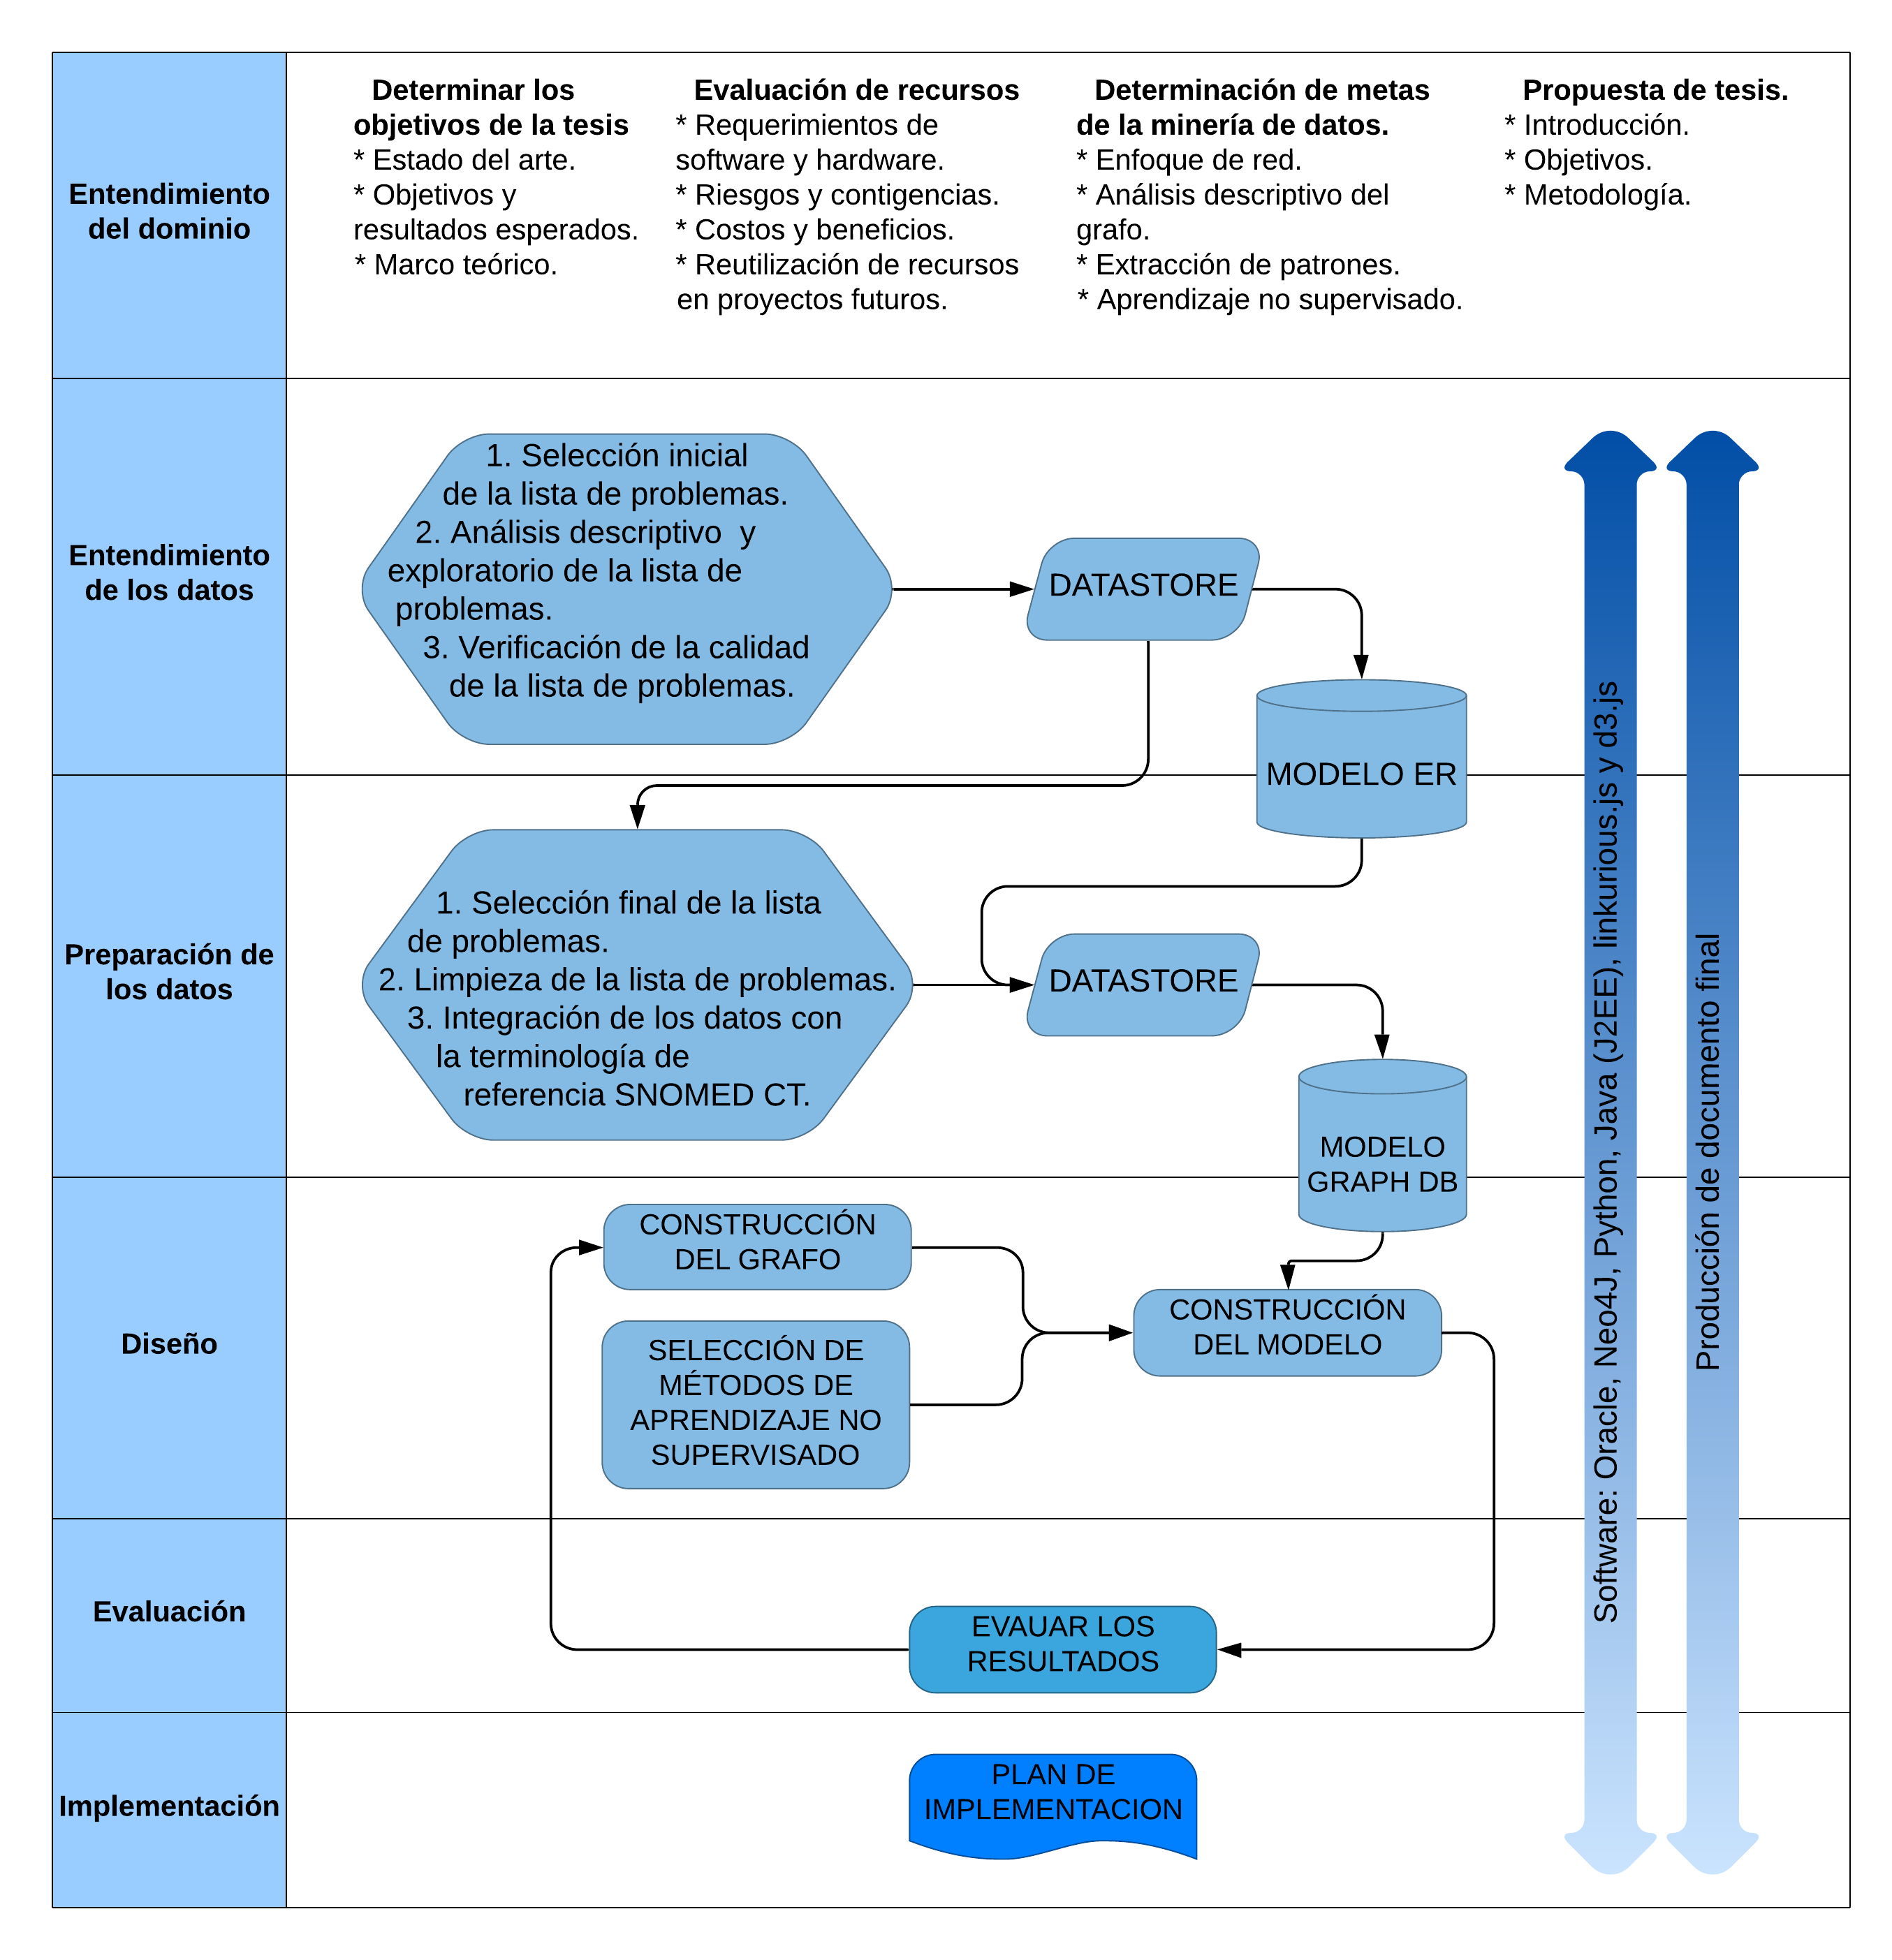
\includegraphics[width=\textwidth]{Metodologia}
\end{figure}

\subsection{Fase 1: Entendimiento del Dominio.} Esta fase fue previa al trabajo de tesis en sí, y el entregable fue la propuesta de tesis. Se compone de la determinación de los objetivos, de las metas de minería de datos y la evaluación de los recursos.

Como está consignado en el primer capítulo introductorio, el objetivo es la construcción de una taxonomía de problemas, cuyas relaciones están ponderadas por su co-ocurrencia en las listas de problemas de los pacientes y sus relaciones jerárquicas con Snomed CT. Para alcanzar dicho objetivo, establecí que la meta de minería de datos es representar el conocimiento en un enfoque de red, y a partir del análisis de la red realizar la construcción jerárquica de grupos o clasificaciones de los problemas.

Para realizar esta tesis, el \acrshort{HIBA} proporcionó el acceso a los datos de la lista de problemas y la terminología. En términos de hardware, el \acrshort{HIBA} proporcionó el acceso a un servidor con las siguientes características:

<< Características del servidor >>

\subsection{Fase 2: Entendimiento de los datos.} Esta fase inicia con la recolección de los datos y procede con las actividades que permitan familiarizarse con ellos. El entregable se encuentra en la primera sección del capítulo 3 y contempla un análisis descriptivo para determinar la calidad de los datos de la lista de problemas, la existencia de valores atípicos (\textit{outliers}) y la construcción de contextos interesantes que permitan la formulación de hipótesis.

\subsection{Fase 3: Preparación de los datos.} Esta fase se compone de la extracción de los datos desde el modelo ER, limpieza y transformación de los datos con los que se realizan los experimentos. El entregable es el conjunto de datos de entrenamiento y validación. El conjunto de entrenamiento contiene los registros de problemas previos al 2017. El conjunto de validación contiene los registros que ingresaron a la \acrshort{HCE} en el 2017 y cuyos pacientes tengan una lista de problemas no vacía.

\subsection{Fase 4 y 5: Diseño y evaluación.} Esta fase es iterativa, y se compone de varios ciclos para refinar el modelo de agrupamiento, durante estos ciclos se realizan las siguientes tareas:
\begin{itemize}
\item Construcción del grafo: Determinación del modelo de datos y carga de la base de datos de grafos. Usando los datos de entrenamiento se obtiene un grafo que conecta los problemas a partir de las co-ocurrencias en los pacientes y las relaciones dadas por la terminología de referencia Snomed CT. Los vértices son etiquetados con información contextual: ámbito o nivel de asistencia, grupo etario y área jerárquica.  

\item Estudio de los patrones en la red: Evaluar la red en un contexto de red libre de escala. El entregable es la caracterización de la red.

\item Aprendizaje no supervisado: Identificación de grupos o \textit{clusters} significativos que comparten patrones comunes de atributos y relaciones. Cada uno de los vértices que contiene el \textit{cluster} tiene calculada las medidas de centralidad para entender su influencia dentro de la red.

\item Validación de los resultados: Este paso se encarga de validar la capacidad predictiva de los modelos de agrupamiento del aprendizaje no supervisado. La hipótesis es que los vértices que pertenecen al mismo \textit{cluster} permiten completar los problemas faltantes en la lista de los problemas de los pacientes del conjunto de datos de validación. 

Son evaluadas por separado la capacidad predictiva del grafo y la de un subgrafo generado sólo con las relaciones por la co-ocurrencia en los pacientes y los vértices de los problemas, es decir sin SNOMED CT. También son evaluadas las capacidades predictivas filtrando el contexto: ámbito o nivel de asistencia, grupo etario y área jerárquica.
 \end{itemize}
 
\subsection{Fase 6: Implementación.} En la última fase organizo los datos y redacto el documento final de la tesis. El plan de implementación en la organización de los datos y los servicios de terminología del acrshort{HIBA} no hacen parte de los entregables de esta tesis.

\section{Algoritmos de aprendizaje no supervisado}
El paquete igraph\cite{igraph} de Python ofrece una variedad de algoritmos para realizar aprendizaje no supervisado. Sin embargo, por el tamaño del grafo algunos algoritmos son imposibles de usar en la práctica. Por ejemplo, el método \textit{leading edge betweenness} para detectar comunidades tiene una complejidad $O(|E||V|^2)$ en el peor caso (donde $|V|$ número de vértices y $|E|$ número de aristas). Para procesar el grafo de esta propuesta de trabajo se necesitaría 181.93 años. Los detalles de otros algoritmos en este paquete para la generación de comunidades se encuentran en la tabla \ref{algoritmos_igraph}.

\begin{table}[tbp]
\centering
\caption{Algoritmos de aprendizaje no supervisado del paquete igraph}
\label{algoritmos_igraph}
\begin{threeparttable}
\begin{tabularx}{\textwidth}{@{}XXXX@{}}
\toprule
Algoritmo & Observaciones & Complejidad\tnote{1}  & Cálculo de tiempo de ejecución\tnote{2} \\ \midrule
\textit{spinglass} & Comunidades basadas en la física estadística & No especificado &  \\
\textit{leading} \newline  \textit{eigenvector} & Comunidades basadas en matrices de autovectores & $O(|E|+|V|^2*steps)$, donde “steps” es atributo del algoritmo & 6.86 segundos \\
\textit{walktrap} & Comunidades basados en caminos aleatorios & $O(|E||V|^2)$ en el peor caso, $O(|V|^2 log|V|)$ en promedio, & 181.93 años en el peor caso, 38 segundos en el caso promedio \\
\textit{edge} \newline \textit{betweenness} & Comunidades basados en la métrica de centralidad intermediación & $O(|E||V|^2)$ en el peor caso & 181.93 años en el peor caso \\
\textit{fast greedy} & Comunidades basadas en optimización de la modularidad & $O(|E||V|log|V|)$ en el peor caso, $O(|E|+|V|log^2|V|)$ en promedio & 22.84 minutos en el peor caso, 0.0011 segundos en promedio \\
\textit{multilevel} & Comunidades mediante la optimización de la modularidad multinivel & En promedio lineal en grafos dispersos & 0.00064 segundos en promedio \\
\textit{label} \newline  \textit{propagation} & Comunidades basadas en la propagación de etiquetas & $O(m+n)$ & Depende del tamaño de la matriz resultante. \\
\textit{infomap} & Estructuras de comunidades que minimizan el valor esperado & No especificado &  \\ \bottomrule
\end{tabularx}
\begin{tablenotes}
    \item[1] donde $|V|$ número de vértices, $|E|$ número de aristas.
    \item[2] Cálculos basados en números de instrucciones por segundos en un procesador AMD Athlon FX-60 (Dual Core) Reloj 2.6 GHZ = 22150 MIPS.
  \end{tablenotes}
\end{threeparttable}
\end{table}

Seleccioné los siguientes algoritmos para realizar todos los experimentos de aprendizaje no supervisados, teniendo en consideración la complejidad computacional y escogiendo un representante de cada uno de los tipo de algoritmos mencionados en el capítulo anterior (divisivos, aglomerativos y optimización).

\subsection{Algoritmo: \textit{leading eigenvector}}\cite{Newman2006FindingMatrices.} 
\begin{itemize}
\item Complejidad: $c|V|^2 + |E|$
\item Tipo de algoritmo: Optimización
\end{itemize} 
El algoritmo \textit{Leading Eigenvector} para detectar estructura de comunidades fue implementado por igraph usando un algoritmo recursivo que divide la red maximizando la modularidad respecto a la red original. 
 
Los métodos basados en este enfoque han tenido excelentes resultados en test estandarizados. Desafortunadamente, la optimización exhaustiva de la \textbf{modularidad} requiere grandes esfuerzos computacionales, incluyendo algoritmos voraces (\textit{greedy}), enfriamiento simulado (\textit{simulated annealing}) y optimización extrema (\textit{EO}). El algoritmo desarrollado por Newman tiene un enfoque diferente, en el cual se reescribe la función de \textbf{modularidad} en términos de la matriz, lo cual permite expresar la tarea de optimización como un problema espectral en el álgebra lineal. Este enfoque lidera una familia de algoritmos rápidos para detectar comunidades que producen resultados competitivos con los mejores métodos previos.
 
\subsection{Algoritmo: \textit{multilevel}}\cite{Blondel2008FastNetworks} 
\begin{itemize}
\item Complejidad: ``lineal'' cuando  $|V|$ es aproximadamente $|E|$, el algoritmo sugiere que podría ser cuadrática con los grafos completamente conectados.
\item Tipo de algoritmo: Aglomerativo
% * <mariad.avila@hospitalitaliano.org.ar> 2017-07-01T19:50:42.851Z:
% 
% Definir grafo completamente conectado
% 
% ^.
\end{itemize}
El tamaño típico de las grandes redes como las redes sociales, las redes telefónicas móviles o la web, ahora se cuenta en millones cuando no miles de millones de vértices y en este escala se demanda nuevos métodos para recuperar información a partir de su estructura. Un enfoque prometedor consiste en la descomposición de redes en subunidades o comunidades. La identificación de estas comunidades es de crucial importancia ya que pueden ayudar a descubrir modulos funcionales desconocidos a priori tales como tópicos en redes de información o ciber comunidades en redes sociales. Ademas, las meta redes resultantes, cuyos vértices son comunidades, pueden ser usadas para visualizar la estructura de la red original.
 
El algoritmo \textbf{multilevel} encuentra particiones con alta \textbf{modularidad} en grandes redes en poco tiempo y despliega una completa estructura de comunidad jerárquica para una red, dando así acceso a diferentes resoluciones de una detección de comunidades. El algoritmo se divide en dos fases que se repiten iterativamente. Asume que se empieza con una red ponderada de $N$ vértices. Primero, se asigna una comunidad diferente a cada vértice de la red. De esta manera, en esta partición inicial hay tantas comunidades como vértices. Entonces, por cada vértice $i$ se evalúa si mejora la \textbf{modularidad} al cambiar la comunidad asociada al vértice $i$ por las comunidades en las que están cada uno de vértices adyacentes a él. El vértice $i$ es entonces puesto en la comunidad en la cual la modularidad es máxima y positiva. Si no se obtiene una ganancia positiva, entonces el vértice $i$ se mantiene en su comunidad original. Este proceso es aplicado repetidamente y de manera secuencial para todos los vértices hasta que no se puede lograr ninguna mejora.
 
\subsection{Algoritmo: \textit{label propagation}}\cite{Raghavan2007NearNetworks.}
\begin{itemize}
\item Complejidad: $|V| + |E|$
\item Tipo de algoritmo: Divisivo
\end{itemize}
Cada vértice es iniciado con una etiqueta. En cada iteración del algoritmo se usa una función uniforme para determinar las aristas que son eliminadas, en el siguiente paso cada vértice adopta la etiqueta que es mayoritaria en los vértices adyacentes. A medida que las etiquetas se propagan a través de la red de esta manera, grupos de nodos densamente conectados constituyen un consenso en sus etiquetas. La condición de parada puede ser que se llegue a la convergencia, es decir que la mayoría de los vecinos de cada vértice tengan la misma etiqueta que dicho vértice, o simplemente por una cantidad de iteraciones prefijada. Al final del algoritmo, los nodos con la misma etiqueta son conectados como comunidad. Las ventajas de este algoritmo sobre otros métodos es su simplicidad y su efectividad en el tiempo. El algoritmo usa la estructura de la red para guiar su progreso y no optimiza alguna métrica específica. Además, el número de comunidades y sus tamaños no son conocidos a priori y son determinados cuando finaliza el algoritmo.
 
Aunque las redes con una sola comunidad satisface el criterio de parada, romper los enlaces aleatoriamente permite que se generen subgrafos disjuntos, evitando así que la misma etiqueta se propague por todo el grafo. En el caso de redes homogéneas que no tienen estructura de comunidades, el algoritmo identifica la red como una sola comunidad.

\section{Métricas de evaluación de resultados}
Teniendo en cuenta las directrices de recuperación de información \cite{Manning2008IntroductionRetrieval,Hersh1994OHSUMED:Research}, el conjunto de validación tiene tres componentes: 

\begin{itemize}
\item \textbf{El conjunto de pruebas}: se conforma de los problemas registrados previamente y los valores del contexto (nivel asistencia, grupo etario y área jerárquica), que representan la \textit{query}, y el problema a predecir que representa la respuesta correcta
\item \textbf{Los conceptos de Snomed CT a ser recuperados}: la lista previa de problemas permite identificar los subgrafos, y los valores de contexto permiten filtrar los vértices. De esta manera, creo una \textbf{lista de sugerencias} por cada uno de los registros del conjunto de pruebas.
\item una medida de relevancia por cada par de \textit{query}-concepto recuperado, esta medida es la \textbf{transitividad} o la \textbf{distancia semántica}, y permite un ordenamiento de los resultados. Estas medidas están definidas en el capítulo introductorio.
\end{itemize}

La evaluación que planteo en este trabajo, mide si los subgrafos que se forman a partir de los \textit{clusters}, y que usan la lista de problemas previas al 2017 y los contextos para su selección y filtrado (\textbf{lista de sugerencias}), permiten predecir los problemas registrados en el 2017.

La precisión y la exactitud (\textit{accuracy}) son obtenidas para evaluar la capacidad del modelo de obtener resultados relevantes. Estas medidas están definidas como:

\begin{equation}
Exactitud = \frac{\text{Verdaderos positivos}+\text{Verdaderos negativos}}{\text{Total de los datos}}
\end{equation}

\begin{equation}
Precision = \frac{\text{Verdaderos positivos}}{\text{Verdaderos positivos}+\text{Falsos positivos}}
\end{equation}

Teniendo en cuenta que las listas de sugerencias son de un tamaño $n$ ordenados según la relevancia, la exactitud suma los verdaderos positivos, que son los casos en los que la lista de sugerencia contiene la respuesta correcta, y los verdaderos negativos, que son los casos en los que la lista de sugerencias esta vacía y el problema a predecir no está dentro de los conceptos de Snomed CT a ser recuperados, y los divide en la totalidad de los datos de prueba. La precisión evalúa cuántas veces la lista de sugerencias no vacía tiene la respuesta correcta, divido las veces que se dió una respuesta positiva. Debido a que la lista de sugerencias es de tamaño $n$ La medida es llamada precisión al $n$ o $P@n$ y exactitud al $n$ o $Acc@n$.






